\chapter{Tests et résultats}

\noindent
L'intégralité du logiciel de monitoring et les composants matériels ont été testés ensemble afin d'évaluer la solution produite au cours de ce mémoire. Malheureusement, le prototype n'a pas pu être testé en conjonction avec l'infrastructure du CERHIS. À la place, les tests ont été réalisés dans un réseau domestique/\textit{Home Area Network} (HAN). Les résultats obtenus ici peuvent ne pas refléter entièrement ceux qui seraient observés dans le réseau local de CERHIS. En effet, les deux réseaux présentent les différences suivantes :

\vspace{0.2cm}

\begin{itemize}
  \item Le réseau domestique est caractérisé par une multitude de dispositifs de types divers tels que des smartphones, des décodeurs TV, des appareils de streaming sans fil et des ordinateurs. Le réseau de CERHIS se compose principalement de tablettes, du serveur, des points d'accès et potentiellement du contrôleur de charge solaire MPPT. Les différents dispositifs peuvent agir différemment lorsqu'ils reçoivent des requêtes PING ou ARP. De plus, les topologies distinctes peuvent avoir un impact sur le délai des réponses, ce qui peut aussi influencer le monitoring des appareils.

  ~

  \item Le réseau domestique ne possède aucun serveur similaire à celui utilisé par CERHIS. Un Raspberry Pi 3B a été employé pour jouer le rôle du serveur de CERHIS et les \textit{node\_exporter} et \textit{process-exporter} ont été configurés dessus. En revanche, contrairement à la situation du serveur de CERHIS, presque aucun trafic de données dans le réseau domestique n'était dirigé vers ce Raspberry. Cela peut aussi avoir une incidence sur les résultats du test.

  ~

  \item La couverture et la qualité des réseaux mobiles en Belgique sont différentes de celles de la République Démocratique du Congo. Puisque le prototype n'utilise que le réseau 2G, la disparité ne devrait pas être frappante. Tout de même, une couverture moins bonne peut avoir un impact sur les capacités du prototype à se connecter au réseau et à transmettre des informations.

  ~

  \item Finalement, le nombre de dispositifs connectés dans le réseau domestique varie en fonction du moment de la journée. Cela est particulièrement vrai pour les smartphones qui se déconnectent lorsqu'ils ne se trouvent plus dans la maison. Le réseau de CERHIS est plus stable, les tablettes sont assignées au centre hospitalier et ne devraient pas quitter les lieux. Cela a un impact sur le nombre d'alertes produites au cours d'une journée, ce qui peut influencer le fonctionnement du système. (Principalement la taille de la base de données et la consommation énergétique)
\end{itemize}

~

\noindent
Malgré ces différences, le réseau domestique offre tout de même la possibilité de mettre à l'épreuve le prototype. En effet, le test effectué sur cet environnement permet de vérifier qu'aucune erreur majeure n'a été commise dans la conception de ce dernier. En outre, un ensemble de métriques surveillées est utilisé pour définir le comportement de base du prototype. Ces métriques seront particulièrement intéressantes à l'avenir pour comparer les résultats obtenus ici avec ceux d'un futur test réalisé avec l'infrastructure de CERHIS.

\section{Définition de l'environnement}

\noindent
Avant de présenter les résultats, l'environnement et les conditions du test doivent être spécifiés afin que les résultats puissent être correctement interprétés. Le réseau domestique surveillé était composé des dispositifs suivants :

\begin{itemize}
  \item Modem sans fin Compal CH7465LG-TN (Modem Telenet)
  \item 1 décodeur TV (Telenet)
  \item 1 boîtier multimédia Android
  \item 1 Google Chromecast
  \item 2 ordinateurs (Windows 10)
  \item 1 Access point (Telenet)
  \item 3 Smartphones (Android 10.0)
  \item 1 smartphone (Android 8.0)
  \item 1 Radio Internet
  \item 1 Raspberry Pi 3B+ (joue le rôle du serveur de CERHIS)
\end{itemize}

~

\noindent
À cette liste s'ajoutent encore quelques dispositifs qui n'ont pas été monitorés, tels que deux ordinateurs portables supplémentaires. Ces machines ont été déconnectées du réseau avant que le mappage soit effectué. Elles n'ont pas été monitorées afin de vérifier si leurs connexions intermittentes affecteraient la surveillance des autres dispositifs. Ceci permet de simuler la situation où un technicien connecte momentanément son appareil au réseau local du centre hospitalier.

~

\noindent
Les fichiers de configuration des \textit{exporters} sont inclus avec le code développé au cours de ce mémoire. La plupart des paramètres ont été conservés par défaut. Un processus Python sans fin a aussi été lancé dans le Raspberry Pi 3B+ afin que le \textit{process-exporter} puisse recueillir des informations dessus.

~

\noindent
Ceci reprend l'entièreté de l'environnement du réseau domestique. Le client de monitoring utilisé correspond à celui qui a été développé au long de ce mémoire. Pour rappel, il est constitué par les composants suivants :


\begin{itemize}
  \item Raspberry Pi 2B
  \item SIM800L + carte SIM Thingstream
  \item XL4015
  \item Le nouveau boîtier avec ventilateur
\end{itemize}
\vspace{0.1cm}
\noindent
L'application de monitoring présenté dans la section \ref{sec:client} était exécutée sur ce Raspberry Pi 2B.

~

\noindent
Pour déployer le serveur de la solution de monitoring, la Google Cloud Platform\cite{google_cloud} a été utilisée. Une instance d'une machine virtuelle tournait le client MQTT et l'application de Grafana, et une instance MySQL a été employée pour la base de données. Il n'y a aucune raison particulière attachée à l'utilisation de cette plateforme au lieu de AWS ou Azure. Des instances dans les autres plateformes pourraient être exploitées avec le même effet. De façon similaire, un serveur privé pourrait être également employé pour déployer cette même application.

~

\noindent
La figure \ref{fig:test_deploy} illustre la manière dont la solution a été déployée afin de réaliser ce test. Un service \textit{node\_exporter} a également été configuré sur le Raspberry Pi 2B exécutant le code du client de monitoring. Cet exporter a permis de collecter de nombreuses métriques sur le fonctionnement de celui-ci, comme la température et l'utilisation du CPU. La section suivante reprend les résultats du test.

\begin{figure} [ht!]
  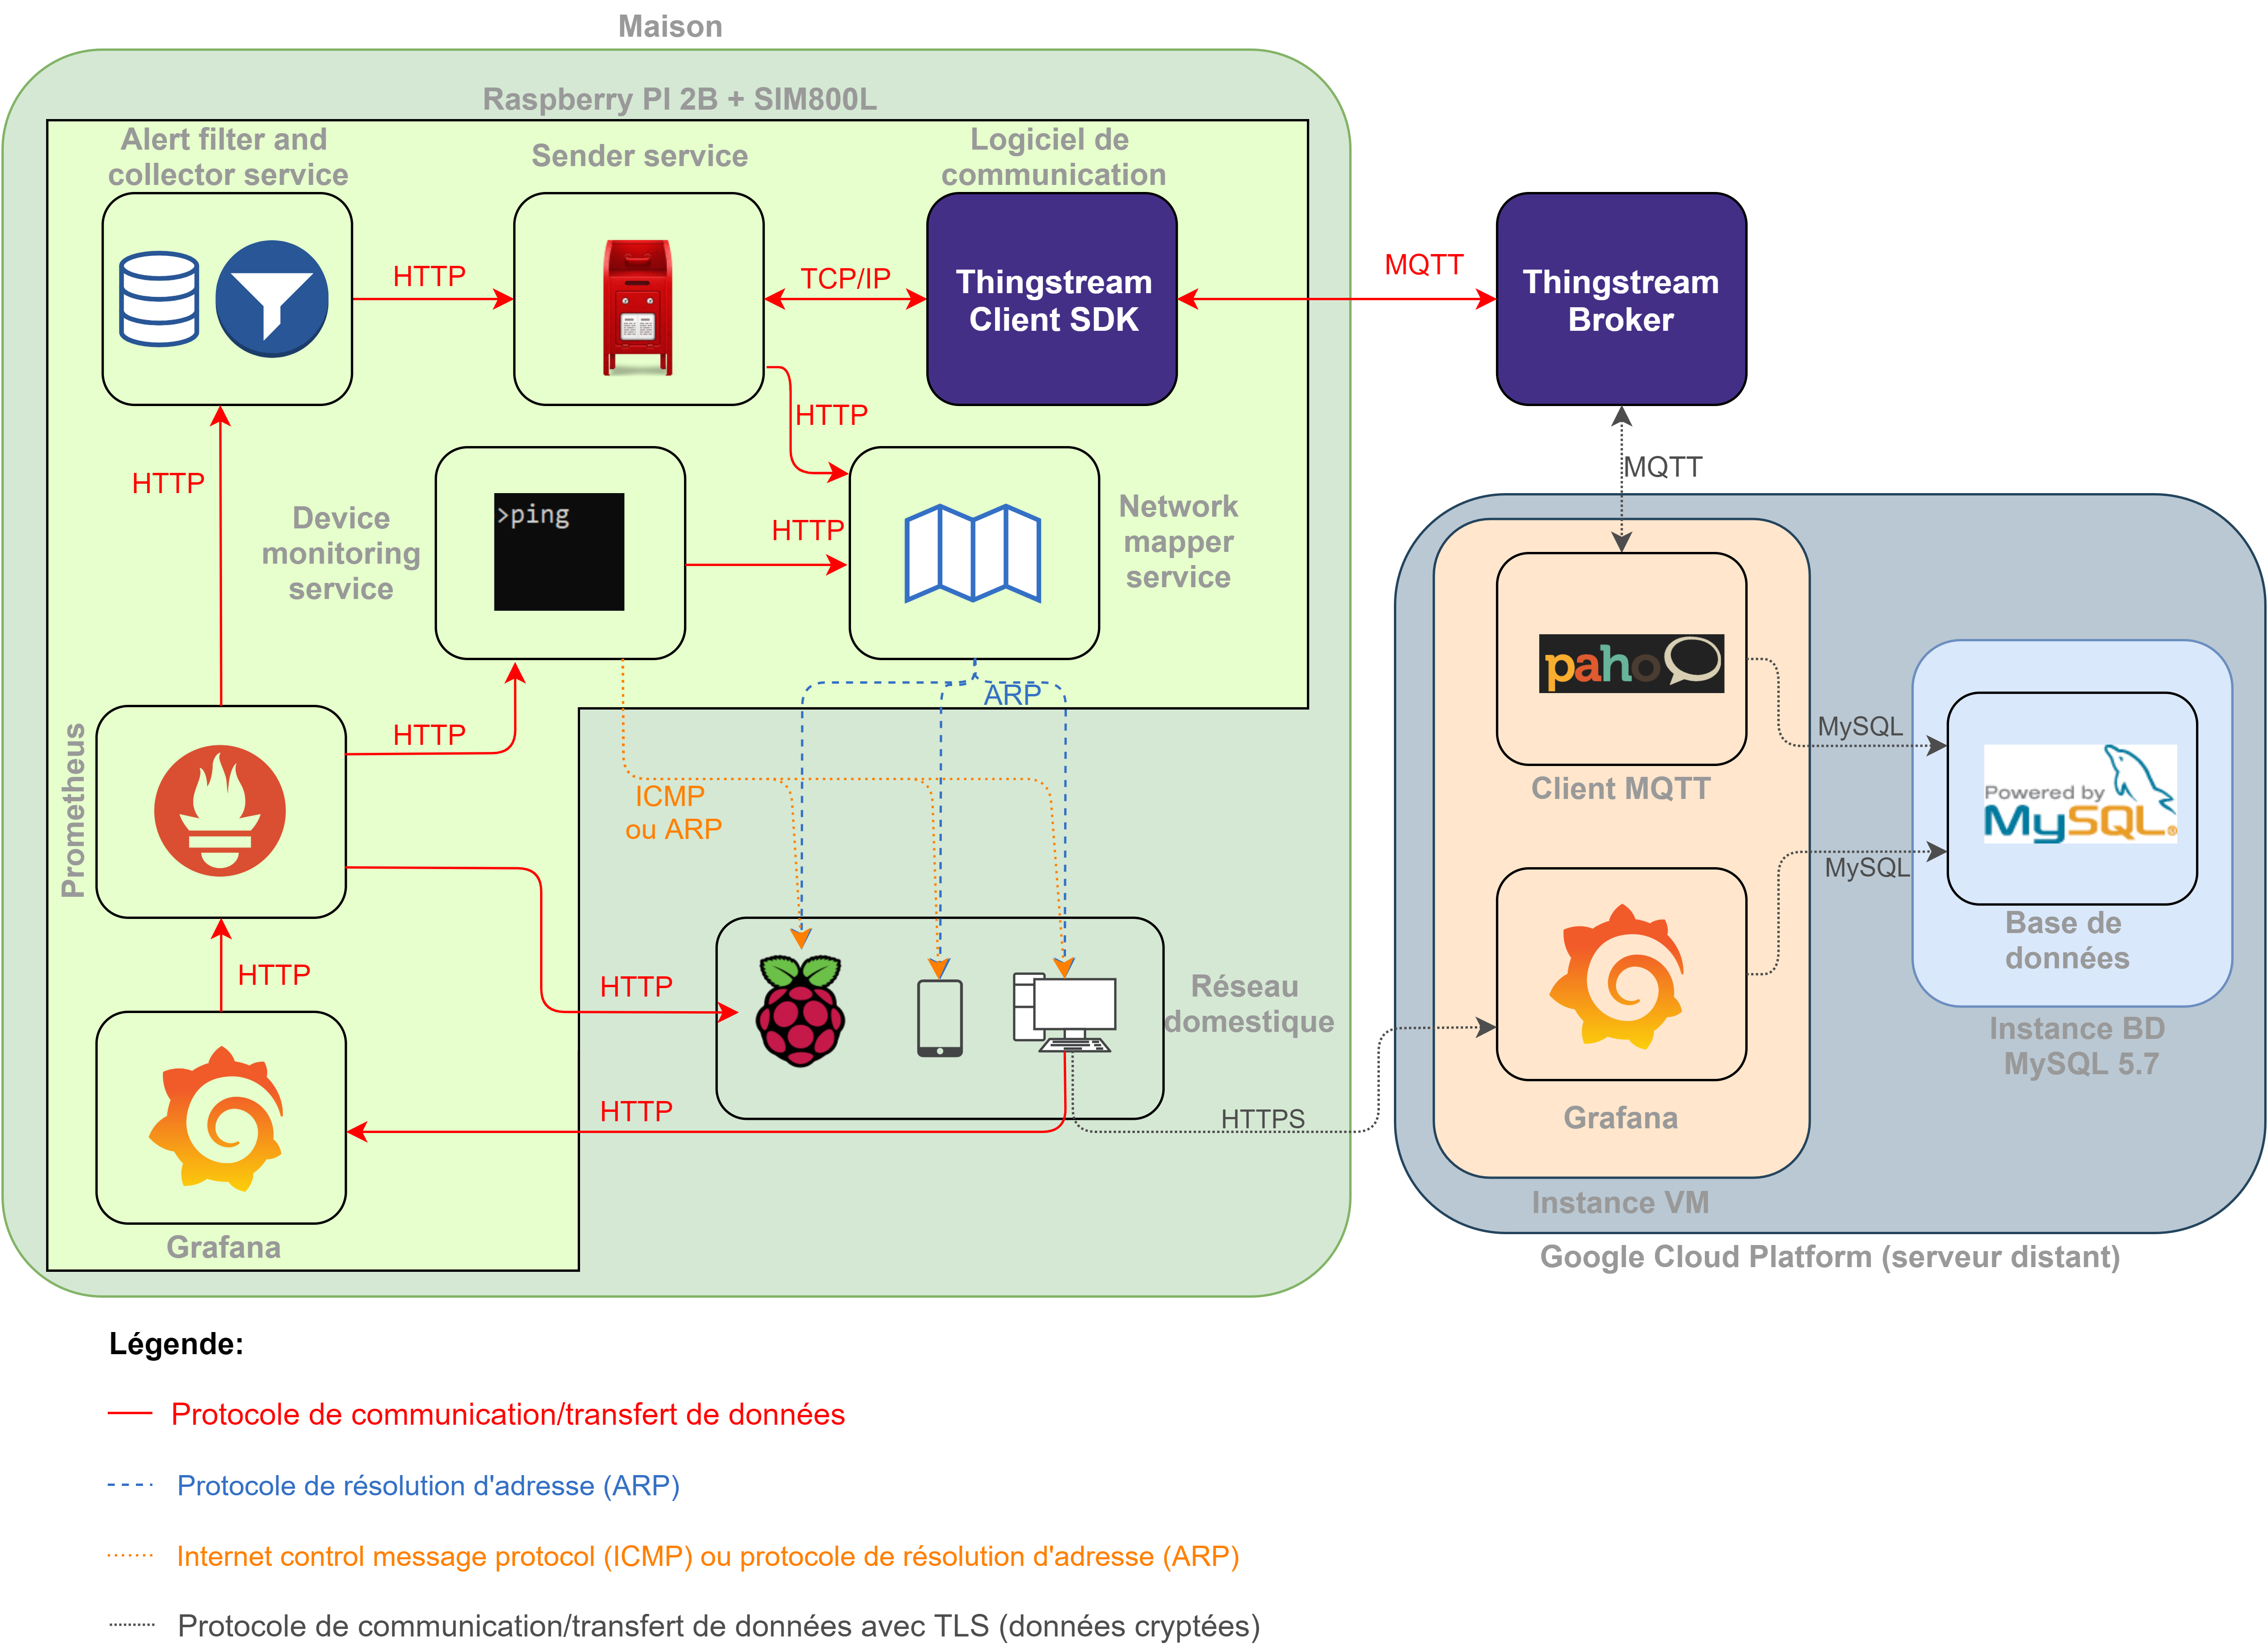
\includegraphics[width=\textwidth]{img/tests/test_env.png}
  \caption{Architecture complète de l'environment de tests}
  \label{fig:test_deploy}
\end{figure}


\section{Résultats}

\noindent
Le prototype ainsi que toute la solution de monitoring ont été testés pendant une période de 3 semaines et demie en continu. Cependant, la solution de communication a été éteinte après 6 jours (ceci sera expliqué plus tard). Malgré cela, la partie restante de la solution de monitoring a continué à fonctionner, seulement les avertissements par SMS et les données sur le serveur ont été impactées.

\subsection{Consommation énergétique}

\noindent
La première métrique du prototype surveillée fût la consommation énergétique. Connaître sa consommation est important afin de correctement dimensionner la capacité de la batterie requise pour celui-ci. Le tableau \ref{tab:conso} reprend les mesures qui ont été prises selon les situations suivantes :
\vspace{0.1cm}
\begin{itemize}
  \item Fonctionnement normal (tous les services de monitoring en cours, tous les composants sont utilisés)
  \item Fonctionnement normal, mais sans ventilateur
  \item Fonctionnement normal, mais sans ventilateur et sans SIM800L (mais avec le XL4015)
  \item Seulement le Raspberry (tous les services toujours en cours, mais un chargeur de 5V a été directement connecté au Raspberry. Le step-down n'a donc pas été utilisé)
\end{itemize}


\begin{table}[ht!]
  \centering
\begin{tabular}{@{}lccc@{}}
\toprule
\textbf{Situations}                                                                  & \textbf{Min} & \textbf{Max} & \textbf{Moyenne} \\ \midrule
\vspace{0.1cm}
\textbf{Normal}                                                                      & 2.5W         & 2.6W         & 2.53W            \\
\vspace{0.1cm}
\textbf{Sans ventilateur}                                                            & 2.3W         & 2.3W         & 2.3W             \\
\vspace{0.1cm}
\textbf{\begin{tabular}[c]{@{}l@{}}Sans ventilateur \\ et sans SIM800L\end{tabular}} & 2.1W         & 2.2W         & 2.14W            \\
\vspace{0.1cm}
\textbf{\begin{tabular}[c]{@{}l@{}}Seulement le \\ Raspberry Pi\end{tabular}}        & 1.6W         & 1.7W         & 1.66W            \\ \bottomrule
\vspace{0.1cm}
\end{tabular}
\caption{Consommation énergétique du prototype selon différentes situations}
\label{tab:conso}
\end{table}

~

\noindent
L'ensemble de ces mesures permet d'inférer plusieurs choses. Premièrement, l'efficacité du step-down utilisé est aux alentours de $76\%$ (voir \ref{eq:conso}). Cette valeur est inférieure à celle documentée dans la fiche technique du XL4015 ($85-90\%$). Cela est probablement dû à plusieurs raisons. En effet, les valeurs mesurées ici ne sont pas très précises ce qui peut influencer les résultats. En outre, un chargeur de 5V a dû être utilisé pour alimenter le Raspberry Pi lorsque sa consommation a été mesuré. En revanche, un chargeur de 12V est utilisé pour alimenter tout le prototype. Les différentes pertes au niveau des chargeurs influencent le résultat. Finalement, des composants de moins bonne qualité peuvent aussi provoquer une chute dans l'efficacité. Deuxièmement, ces mesures permettent d'établir le bilan de la consommation énergétique du prototype. Ce bilan est illustré dans la figure \ref{eq:pie}.

\begin{equation}
  \eta = \frac{\text{énergie utile}}{\text{énergie totale}} = \frac{1.6W}{2.1W} = 0.76
  \label{eq:conso}
\end{equation}

\begin{figure}[ht!]
  \centering
  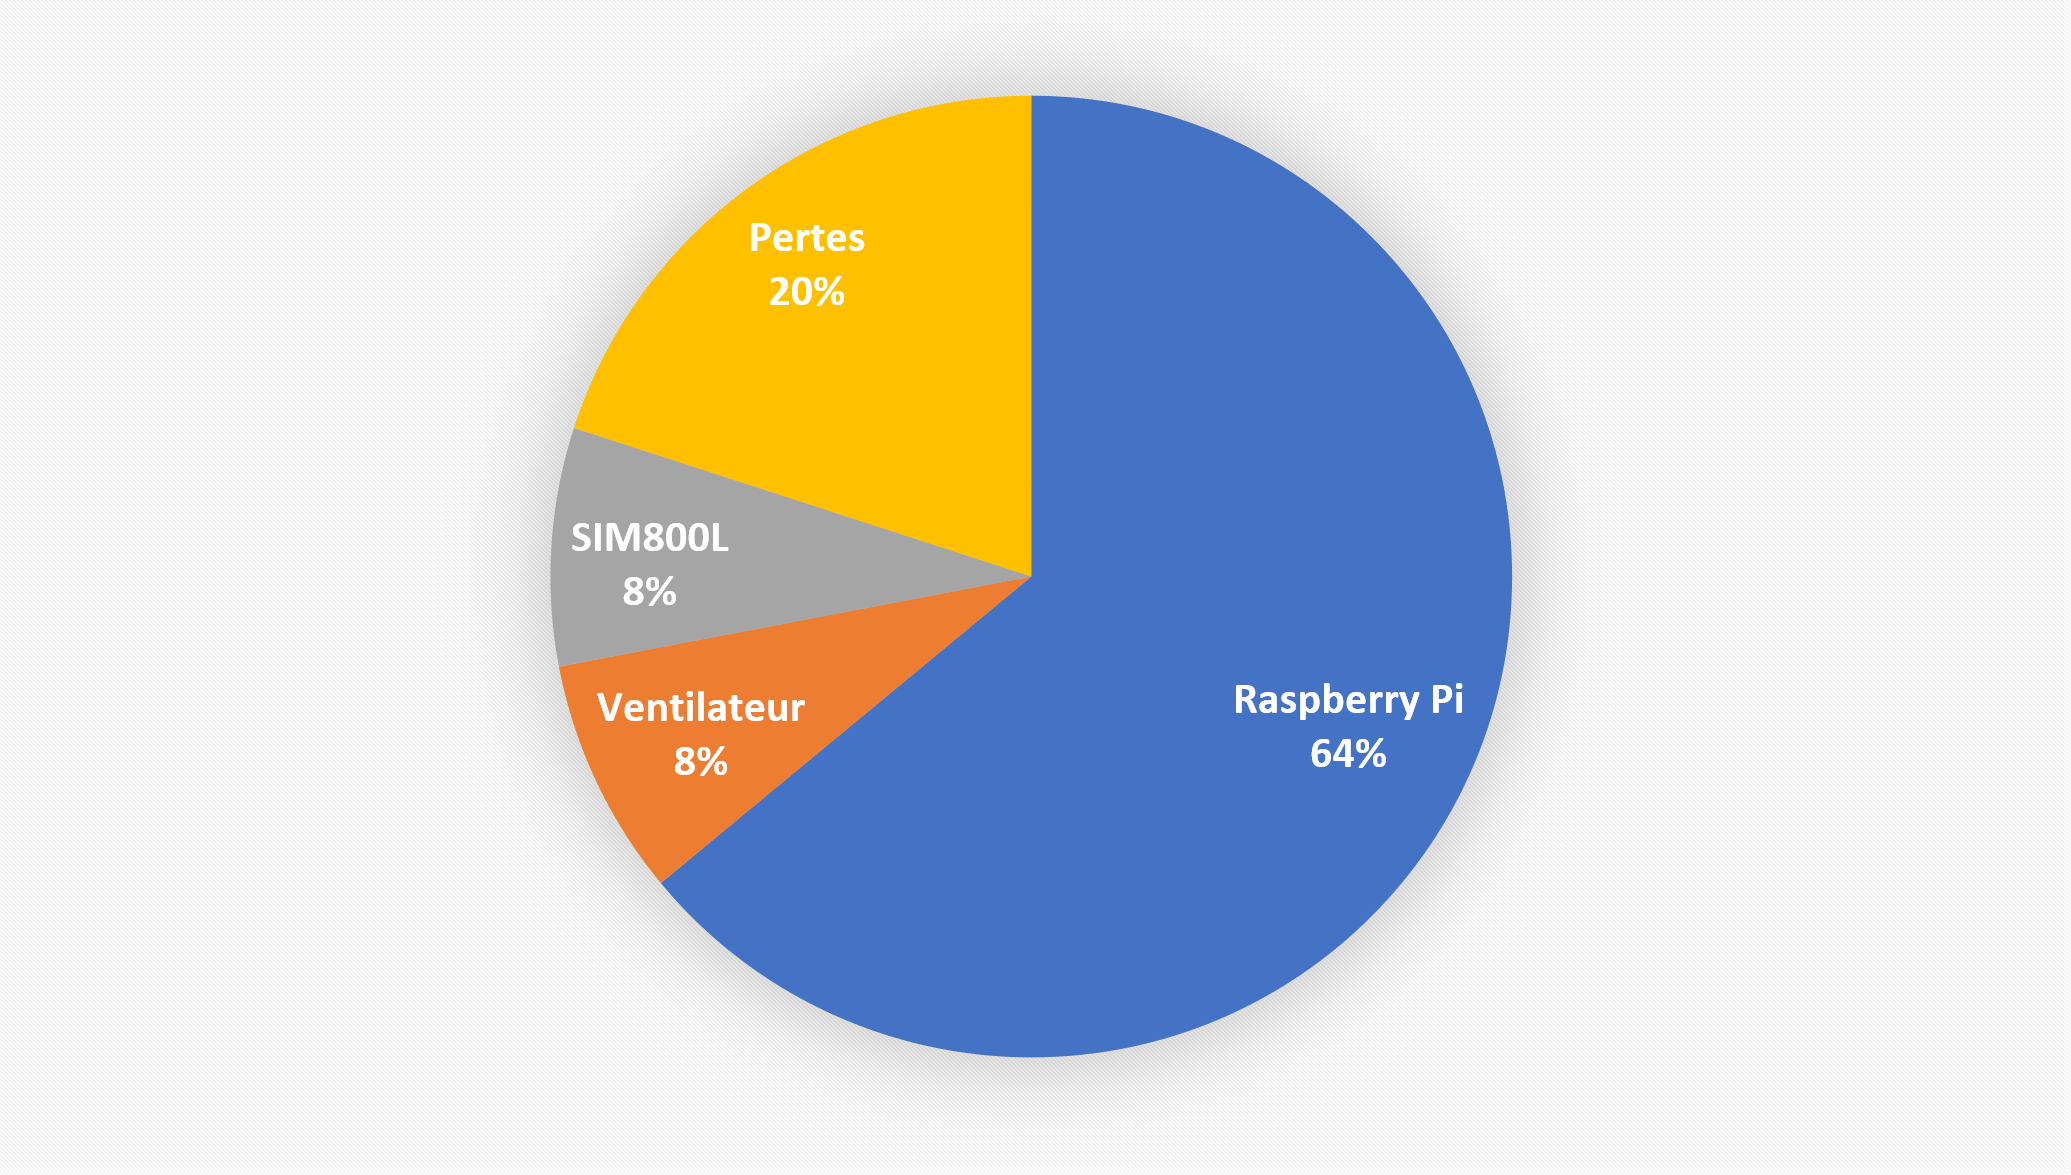
\includegraphics[width=0.8\textwidth]{img/tests/pie_chart.png}
  \caption{Bilan énergétique du prototype}
  \label{eq:pie}
\end{figure}

~

\noindent
Une batterie de 12V et 6Ah devrait suffire pour alimenter le prototype pour un peu plus d'une journée. En revanche, ce temps pourrait être diminué si un technicien accède à l'application de Grafana qui tourne sur le Raspberry. En effet, pendant l'utilisation de ce logiciel, la consommation monte aux alentours de $3.5W$ pendant un court instant. Mesurer le vrai impact de ces piques de consommation n'a pas été possible car le taux de rafraîchissement du wattmètre était très faible. En outre, un phénomène assez similaire est attendu lorsque le SIM800L transmet des informations sur le réseau. Cependant, les limitations du wattmètre n'ont pas permis à nouveau d'obtenir des valeurs à ce sujet. De ce fait, plus de tests devront été réalisés dans le futur par rapport à ces deux cas.

\subsection{Utilisation et température du CPU}

\noindent
Prometheus ainsi que tous les services du logiciel de monitoring se sont montrés peu gourmands en ressources du CPU du Raspberry Pi. Sur les 3 semaines d'exécution, l'utilisation du CPU n'a jamais dépassé les $10\%$ (sur l'ensemble des 4 cœurs). L'utilisation moyenne était entre 1 et $2\%$. Le graphique de la figure \ref{fig:cpu_usage} illustre l'évolution de l'utilisation du CPU au cours de la période de test.

\begin{figure}[ht!]
  \centering
  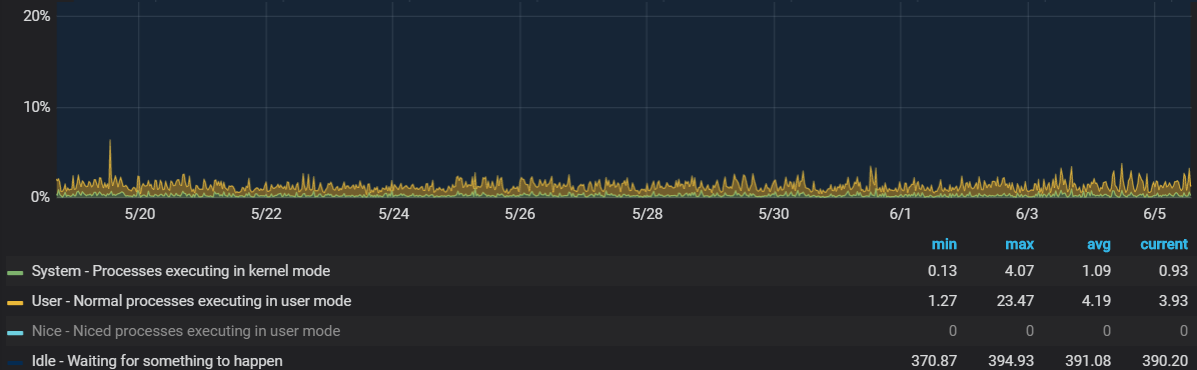
\includegraphics[width=0.87\textwidth]{img/tests/cpu_usage.png}
  \caption{Évolution de l'utilisation du CPU du Raspberry 2B. Les valeurs sur le tableau sont comprises entre 0 et 400 pour cent\textsuperscript{a}}
  \small\textsuperscript{a=} Le Raspberry Pi a quatre cœurs et l'utilisation de chaque coeur est mesurée entre 0 à 100 pour cent. \noindent La valeur sur le tableau correspond à l'addition de la valeur d'utilisation des quatre coeurs.
  \label{fig:cpu_usage}
\end{figure}

%\footnotemark
%\footnotetext{Le Raspberry Pi a quatre cœurs et l'utilisation de chaque coeur est mesurée entre 0 à 100 pour cent. La valeur sur le tableau correspond à l'addition de la valeur d'utilisation des quatre coeurs.}

\begin{figure}[ht!]
  \centering
  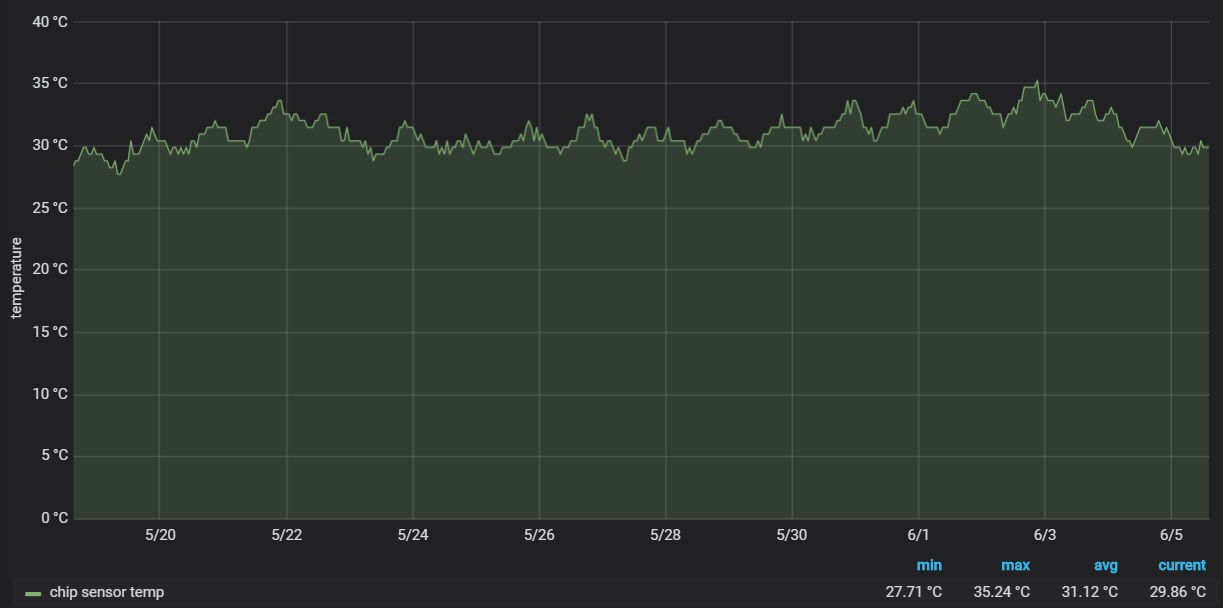
\includegraphics[width=0.87\textwidth]{img/tests/temps.png}
  \caption{Évolution de la température du CPU du Raspberry 2B.}
  \label{fig:cputemp}
\end{figure}


\noindent
L'évolution de la température du CPU est reprise sur la figure \ref{fig:cputemp}. Tout comme dans les tests réalisés précédemment (voir section \ref{sec:protores}), le système de refroidissement du nouveau boîtier contrôle correctement la température du CPU. Il y a une légère augmentation au début du mois de juin, qui atteint son pique aux alentours du troisième jour. Cela est lié à une augmentation de la température ambiante.



\subsection{Détection d'alertes et envoi des messages}

\noindent
Cette partie était la plus complexe à tester. En effet, il est irréaliste de vérifier manuellement l'état de tous les dispositifs du réseau de façon continue sur une période aussi longue. Cela crée un problème puisqu'il n'y a pas un ensemble de données avec lesquel il est possible de comparer ce qui a été mesuré par le prototype. La stratégie pour examiner le fonctionnement de ce composant a dû être modifiée.

~

\noindent
En revanche, il est possible de vérifier manuellement si un message d'alerte envoyée par le prototype correspond aux conditions actuelles de l'infrastructure. C'est donc cette approche qui a été prise. Tous les SMS expédiés par le prototype ont été vérifiés ainsi que les messages transmis au serveur. Pendant les 6 jours où la solution de communication est restée connectée, sur 70 alertes envoyées, une seule s'est révélée être un faux positif. Cette alerte était liée à la disparition de la radio Internet du réseau local, ce qui n'est jamais arrivé. Les données sur le serveur distant permettent de voir qu'à peine trois minutes après sa déconnexion, la radio Internet était à nouveau marquée comme étant présente (voir figure \ref{fig:wrong_alert}).

\begin{figure}[ht!]
  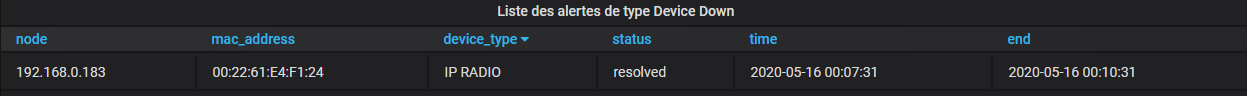
\includegraphics[width=\textwidth]{img/tests/wrong_alert.png}
  \caption{Données de l'alerte qui a été incorrectement signalée}
  \label{fig:wrong_alert}
\end{figure}

~

\noindent
Cette alerte pourrait être liée à une déconnexion momentanée de la radio, mais cela ne peut pas être dit avec certitude. De ce fait, l'erreur est attribuée au prototype. Tout de même, un faux positif sur 70 alertes envoyées correspond à un taux d'erreur de moins de $2\%$, ce qui est très faible. En plus de vérifier la présence de faux positifs parmi les alertes, ce test a également permis d'identifier les problèmes suivants :

\vspace{0.1cm}
\begin{itemize}
  \item Lorsqu'une alerte était en cours et qu'une deuxième était détectée, deux SMS étaient expédiés au technicien malgré le fait qu'un SMS ait déjà été envoyé pour la première alerte. Par exemple, supposons que trois appareils sont déconnectés depuis une heure et que le technicien ait déjà été averti à propos de leur disparition. Si un quatrième dispositif se déconnecte, quatre SMS étaient transmis au technicien, un par appareil absent. Ceci était dû au fait que Prometheus \textit{push} une liste contenant l'entièreté des alertes en cours chaque fois qu'une nouvelle alerte est identifiée. Ce problème a été résolu en ajoutant un filtre dans le service \textit{Alert filter and collector}. Ce dernier vérifie si un message a déjà été envoyé dans le passé et, si c'est le cas, il ne le \textit{push} pas afin d'éviter un SPAM d'avertissements.

  ~

  \item Les données de Prometheus étaient horodatées en fonction du fuseau horaire UTC. En revanche, les données du service \textit{network mapper} étaient horodatées selon le fuseau horaire local. Cela créait une incohérence dans les informations. Ce problème a également été corrigé en horodatant les données du \textit{network mapper} selon le fuseau horaire UTC.

  ~

  \item Certains smartphones Android éteignent le Wi-Fi pendant la nuit dans le but d'économiser de la batterie. Cela s'est produit avec deux des quatre smartphones surveillés. Ce comportement peut généralement être désactivé dans le système d'exploitation. Une autre solution pourrait être de faire taire les alertes de présence pendant la nuit. Cependant, ceci n'a pas été implémenté dans le service de device monitoring.

  ~

  \item Le dernier souci détecté est lié à un bug dans le SDK de Thinsgtream. Le protocole MQTT stipule que si un client et le \textit{broker} n'ont pas communiqué pendant une certaine période, les deux parties doivent échanger un PING pour vérifier que la connexion est toujours active. La durée de cette période est définie à l'aide de la variable \textit{KEEP ALIVE} et elle est configurable. Cependant, le SDK de Thingstream impose que ce temps soit de 5 minutes, indépendamment de la configuration passée. Cela pose un problème puisque chaque PING requiert deux messages qui sont chargés par Thingstream. Sur un mois, cela correspond à un échange de plus de 17000 messages payants rien que pour les PINGs. Ceci se traduira par un coût allant de quatre à presque neuf dollars selon le tarif choisi (voir image \ref{fig:thing_plans}). Après avoir contacté le support technique de Thingstream, ils ont reconnu que c'était une erreur de leur part et que le SDK allait être révisé à l'avenir. Malheureusement, ils n'ont pas donné une date et au temps de l'écriture de ce mémoire, le correctif n'est toujours pas disponible. Cela est la raison pour laquelle le service de connexion a été déconnecté. En quelques jours, le client avait largement dépassé son quota de messages et continuerait à faire de même s'il n'était pas arrêté.
\end{itemize}


\begin{figure}[ht!]
  \centering
  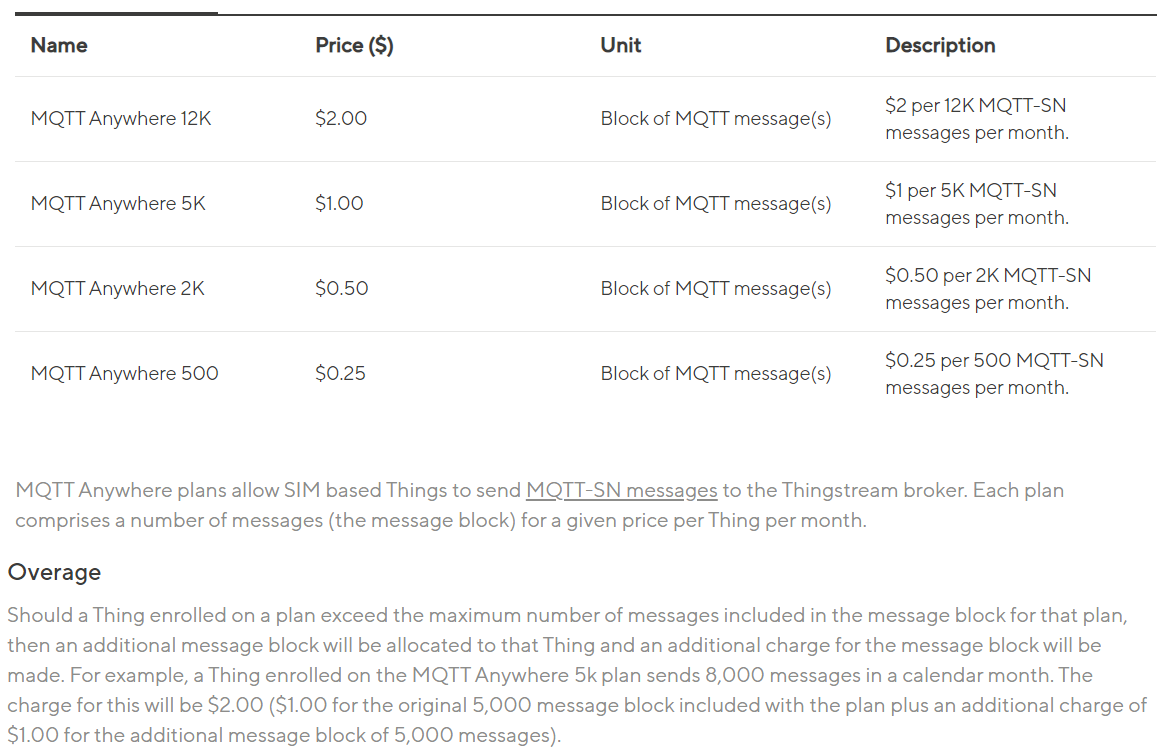
\includegraphics[width=\textwidth]{img/tests/thing_plans.png}
  \caption{Prix des différent tarifs de Thingstream.}
  \label{fig:thing_plans}
\end{figure}


\subsection{Rapidité de la détection d'alertes}


\noindent
La dernière métrique surveillée est la durée requise par le prototype pour détecter et prévenir un technicien à propos de la disparition d'un dispositif. Ce test est facile à effectuer puisqu'il suffit de manuellement déconnecter un appareil du réseau et de compter le temps passé jusqu'à la réception du SMS. En revanche, ce temps n'est pas constant. Le service \textit{device monitoring} ne contrôle la présence des dispositifs qu'une fois par minute. Le temps d'envoi d'un SMS sera plus ou moins long en fonction du délai passé depuis la dernière vérification. De ce fait, les résultats présentés sur le tableau \ref{tab:end_delays} correspondent à une moyenne réalisée sur 10 tests, permettant de mieux visualiser quel sera le temps de réponse moyen du prototype.


\begin{table}[ht!]
  \centering
%\resizebox{\textwidth}{!}{%
\begin{tabular}{@{}lccc@{}}
\toprule
\textbf{Mesures}                                                                  & \textbf{\begin{tabular}[c]{@{}c@{}}Temps moyen \\ (s)\end{tabular}} & \textbf{\begin{tabular}[c]{@{}c@{}}Temps max\\ (s)\end{tabular}} & \textbf{\begin{tabular}[c]{@{}c@{}}Temps min\\ (s)\end{tabular}} \\ \midrule
\textbf{\begin{tabular}[c]{@{}l@{}}Détection \\ dispositif  disparu\end{tabular}} & 56                                                                  & 78                                                               & 41                                                               \\
\vspace{0.1cm}
\textbf{\begin{tabular}[c]{@{}l@{}}Délai configuration\\ Prometheus\end{tabular}} & 120                                                                 & 120                                                              & 120                                                              \\
\vspace{0.1cm}
\textbf{Envoi du SMS}                                                             & 45                                                                  & 49                                                               & 38                                                               \\
\vspace{0.1cm}
\textbf{Total}                                                                    & 221                                                                 & 243                                                              & 206                                                              \\ \bottomrule
\end{tabular}%
%}
\caption{Temps requis pour le prototype pour identifier, générer et envoyer une alerte à propos d'un dispositif qui s'est déconnecté du réseau (Les valeurs des colonnes max et min ne correspondent pas forcément au même test.)}
\label{tab:end_delays}
\end{table}

~

\noindent
Veuillez noter qu'en raison de la configuration actuelle, Prometheus attend toujours deux minutes avant de déclencher une alerte. Ce temps peut être réduit pour obtenir un message plus rapidement, mais cela peut augmenter le nombre de faux positifs. En analysant les données recueillies par Prometheus de plus près, il est possible de constater qu'il faut généralement entre 41 à 78 secondes pour détecter qu'un dispositif est absent du réseau (service \textit{device monitoring}). Ensuite, une fois que les deux minutes se sont écroulées au niveau de Prometheus, entre 38 à 49 secondes sont requises pour que le SMS arrive chez le technicien. Ceci est lié au fait que les messages sont ajoutés dans une file d'attente dans le client de Thingstream. Le SDK retire et traite un message de la file une fois toutes les 30 secondes. Un processus assez similaire a lieu dans le \textit{sender service}, qui patiente une dizaine de secondes avant de tout transmettre au client de Thingstream. Cela permet d'attendre pour vérifier si d'autres alertes doivent également être envoyées. De ce fait, en cas d'alertes multiples, les SMS sont expédiés en premier lieu au client de communication. Cela évite la situation où un SMS d'alerte serait trop retardé à cause de messages à transmettre au serveur distant, car la file d'attente fonctionne sur le principe premier entré, premier sorti (FIFO).

~

\noindent
Finalement, il est possible de conclure que le temps entre le début d'un événement (disparition d'une tablette ou alerte dans le serveur) et la réception d'un SMS sera au maximum de 5 minutes. Cette valeur parait tout à fait raisonnable, mais pourrait encore être optimisée dans le futur. En effet, avec des tests sur l'infrastructure de CERHIS il serait possible de configurer les différents délais afin d'avoir le meilleur compromis entre rapidité, consommation énergétique et fiabilité des alertes.
